% BraTS 2026 Challenge -- Task 1 (Brain Metastases) -- short paper
%
% RULES (verified 2026-07-28 against Synapse wiki syn74274097, page 639582):
%   * 8-10 pages WITHOUT references. Citations do not count toward the limit.
%   * Springer LNCS format (bit.ly/2TEcZNF).
%   * Mandatory sections, in order: Abstract (NO CITATIONS) / Keywords /
%     Introduction / Methods / Results / Discussion / Acknowledgements (optional) /
%     References (must include the citations listed in the Challenge Rules).
%   * Submit via OpenReview: https://openreview.net/group?id=MICCAI.org/2026/Challenge
%     (BraTS-METS subgroup: .../Challenge/BraTS-METS)
%   * You will be asked for the Synapse team name: 3495063
%
% Requires llncs.cls -- see paper/README.md.
\documentclass[runningheads]{llncs}

\usepackage[table]{xcolor}
\usepackage{graphicx}
\usepackage{booktabs}
\usepackage{array}
\usepackage{amsmath}
\usepackage{tikz}
\usetikzlibrary{arrows.meta,positioning}
\usepackage[hidelinks]{hyperref}

\definecolor{famtext}{RGB}{28,74,128}
\definecolor{famrow}{RGB}{233,240,249}
\definecolor{hdrrow}{RGB}{240,240,240}

\begin{document}

\title{Inference-Time Decoding for Brain Metastasis\\ Segmentation: Ensembling, Hysteresis Thresholding,\\ and Post-processing Validation}
\titlerunning{Inference-Time Decoding for Brain Metastasis Segmentation}

\author{%
Soumya Snigdha Kundu\inst{1} \and
Theodore Barfoot\inst{1} \and
Marina Ivory\inst{1} \and
Kabir Hamzah Muhammad\inst{1} \and
Lorena Garcia-Foncillas Macias\inst{1} \and
Jonathan Shapey\inst{1,2} \and
Tom Vercauteren\inst{1}%
}
\authorrunning{S. S. Kundu et al.}

\institute{School of Biomedical Engineering \& Imaging Sciences,
King's College London, London, UK\\
\email{soumya\_snigdha.kundu@kcl.ac.uk}
\and
Department of Neurosurgery, King's College Hospital NHS Foundation Trust,
London, UK}

\maketitle

%%%%%%%%%%%%%%%%%%%%%%%%%%%%%%%%%%%%%%%%%%%%%%%%%%%%%%%%%%%%%%%%%%%%%%%%%%%%%%%
% ABSTRACT -- one paragraph, 6-7 sentences. NO CITATIONS (challenge rule).
\begin{abstract}
Lesion-wise evaluation makes brain metastasis segmentation a joint detection and delineation
problem: lesions contribute equally regardless of volume, while unmatched predictions reduce
lesion-wise overlap scores and detection $F_1$. We investigate how inference-time decoding affects
a standard nnU-Net ResEnc-L system. An unweighted average of three trained models followed by
hysteresis thresholding increased lesion-wise Dice from 0.560, 0.622 and 0.593 to
0.725, 0.766 and 0.746 for WT, TC and ET, respectively, with these two steps accounting for more than four fifths of the observed
improvement. Hysteresis uses a high seed threshold to decide whether a component exists and a
lower threshold to recover its extent, without filtering by component size. On 80 training cases,
false-positive components had higher peak probabilities than missed reference lesions (median
0.96 versus 0.55), and seven tested suppression strategies based on component size or confidence
failed to improve detection without sacrificing true lesions. We also found that post-processing
selected on cases used for training could transfer poorly when it altered component retention: a
cavity rule estimated at $+0.028$ Dice locally produced $-0.016$ on official validation. These
results provide a practical inference-time recipe and caution against treating training-set
post-processing experiments as evidence of held-out improvement.

\keywords{Brain metastases \and Lesion-wise evaluation \and Ensembling \and Hysteresis
thresholding \and False positives \and nnU-Net \and BraTS.}
\end{abstract}

%%%%%%%%%%%%%%%%%%%%%%%%%%%%%%%%%%%%%%%%%%%%%%%%%%%%%%%%%%%%%%%%%%%%%%%%%%%%%%%
\section{Introduction}
\label{sec:intro}

Brain metastases often present as numerous, small and spatially scattered targets, making their
automated delineation substantially different from whole-region tumour segmentation. Earlier
glioma benchmarks that shaped the field scored whole regions~\cite{baid2021}, whereas BraTS-METS
uses lesion-wise evaluation~\cite{bratsmet2023,bratsmet2025,brats2026}. Predicted components are
matched one-to-one to reference components~\cite{grosskopf2026matching}; each matched lesion
contributes equally to the Dice and normalised surface Dice (NSD) averages irrespective of volume,
while unmatched predictions receive zero overlap and count as false-positive detections under the
applicable small-instance evaluation.

This inverts the usual economics. Under volumetric Dice a five-voxel false positive is
negligible; under lesion-wise scoring it costs as much as missing a large lesion. Conversely, a
method that suppresses small components to protect Dice can damage the detection metric the task
is intended to measure. Over the operating range we tested, improvements in detection and
delineation frequently traded off, as quantified in Section~\ref{sec:frontier}.

We began from a standard nnU-Net ResEnc-L~\cite{isensee2021nnunet,isensee2024resenc} baseline and
found repeatedly that changes to the network bought less than changes to how its probabilities
became a label map. Our contributions are:

\begin{enumerate}
\item \textbf{An effective inference-time recipe.} Ensembling as a false-positive dilution
      mechanism, followed by hysteresis decoding, contributes more than four fifths of the total
      Dice improvement over our baseline (Section~\ref{sec:ablation}) without retraining the
      constituent models.
\item \textbf{An analysis of the residual error.} The remaining false positives are confident,
      coherent, isolated and corroborated across independently trained networks. Across seven
      tested suppression strategies, simple component-size and confidence criteria did not
      separate them from true lesions in our models (Section~\ref{sec:fp}).
\item \textbf{An empirical warning for lesion-wise post-processing.} We show how tuning on cases
      used for training can conceal the false-positive cost of rules that retain additional
      components, and quantify one reversal between local and official validation
      (Section~\ref{sec:harness}).
\end{enumerate}

\paragraph{What is and is not novel.} No individual component is new: nnU-Net and its
residual-encoder variants are established~\cite{isensee2021nnunet,isensee2024resenc}, probability
averaging is standard, hysteresis dates to Canny~\cite{canny1986}, and our third member's objective
follows blob loss~\cite{kofler2022blob,kundu2026instance}. The contribution is therefore an
empirical analysis of where performance arose under lesion-wise scoring, together with practical
lessons from the resulting error analysis and validation failures.

%%%%%%%%%%%%%%%%%%%%%%%%%%%%%%%%%%%%%%%%%%%%%%%%%%%%%%%%%%%%%%%%%%%%%%%%%%%%%%%
\section{Methods}
\label{sec:methods}

\subsection{Data}
\label{sec:data}

We use the BraTS-METS 2026 training set~\cite{bratsmet2025,brats2026}: 1295 multi-site cases, each with four co-registered,
skull-stripped sequences (T1, T1-Gd, T2, T2-FLAIR) supplied in \emph{native} space, so voxel
spacing and array dimensions vary across the cohort. Reference labels comprise non-enhancing
tumour core (NETC), surrounding non-enhancing FLAIR hyperintensity (SNFH), enhancing tumour (ET)
and resection cavity (RC). Region prevalence is markedly imbalanced (54\% NETC, 89\% SNFH,
96\% ET and only 13\% RC), which is the principal reason the RC channel is our weakest and is
handled separately below.
% REVIEW TODO: State whether the corrected-label overlay and the later QCed UCSD release were used.
Validation uses the official 179-case set scored on the challenge
server, which runs the organisers' evaluation containers through the MedPerf
platform~\cite{medperf2023}; we never see its reference labels.

We predict four \emph{overlapping} binary regions with independent sigmoids rather than mutually
exclusive classes,
\[
\mathrm{WT}=\{1,2,3\},\quad \mathrm{TC}=\{1,3\},\quad \mathrm{ET}=\{3\},\quad \mathrm{RC}=\{4\},
\]
decoded in the order WT $\rightarrow$ TC $\rightarrow$ ET $\rightarrow$ RC so nested regions
overwrite their parents. This is the \texttt{Dataset007} configuration in our released code.

\subsection{Ensemble members}
\label{sec:members}

The submission averages three ResEnc-L models sharing the residual-encoder plans and the
\texttt{3d\_fullres} configuration (Table~\ref{tab:members}), all trained on all available
data without a held-out fold, a decision whose consequences we return to in
Section~\ref{sec:harness}.

\begin{table}[t]
\centering
\caption{Ensemble members. All are nnU-Net ResEnc-L, \texttt{3d\_fullres}, trained on all data.}
\label{tab:members}
\begin{tabular}{@{}llll@{}}
\toprule
member & data configuration & training objective & role in the ensemble \\
\midrule
TopK        & 4-region  & Dice + top-$K$ BCE          & high-precision base \\
completion  & 6-region  & Dice + top-$K$ BCE          & decorrelated second view \\
CC-loss     & 6-region  & component-weighted fine-tune & high-recall detector \\
\bottomrule
\end{tabular}
\end{table}

% REVIEW TODO: Define the two additional outputs in the 6-region configuration, explain the
% 'completion' member, give the top-K fraction, and state the CC-loss fine-tuning schedule.
The third member is fine-tuned with a connected-component-aware objective that weights each
lesion equally rather than each voxel, following the blob-loss
principle~\cite{kofler2022blob,kundu2026instance}.
It is our strongest detector and our weakest segmenter. Submitted alone it reached small-instance
$F_1$ of 0.429/0.530/0.543, the highest we ever recorded, while its lesion-wise Dice fell to
0.670/0.715/0.691, below the final ensemble; used alone, its additional false positives offset its detection gains. This
tension is precisely what the ensemble exploits.

Inference uses sliding-window prediction with \texttt{step\_size} 0.25 and test-time
augmentation by mirroring, retaining per-region probability maps.

\subsection{Ensembling as false-positive dilution}
\label{sec:ensembling}

The tumour probability map is the unweighted mean over members $m$,
\[
\bar{p}_r(x) \;=\; \tfrac{1}{3}\sum_{m=1}^{3} p_r^{(m)}(x), \qquad
r \in \{\mathrm{WT},\mathrm{TC},\mathrm{ET}\}.
\]

The mechanism is asymmetric, and the asymmetry is the point. A detection supported by all three
members retains a high mean; one idiosyncratic to a single member is divided by three and falls
below the decision threshold. Averaging the high-recall CC-loss member into two cleaner models
reduced false positives from \textbf{1.66 to 0.85 per case} on the local 80-case harness while retaining its corroborated true
detections. Dice and $F_1$ rose \emph{together} rather than trading in this comparison, making the ensemble
more than a variance-reduction convenience in our system.

The resection cavity is treated separately. RC was typically a single large structure in our data, and ensembling gave no measurable benefit:
a two-model RC average moved lesion-wise Dice from 0.630 to 0.628.
We therefore take RC from the CC-loss member alone, threshold at 0.5, and retain only the largest
connected component.

\subsection{Hysteresis decoding}
\label{sec:hysteresis}

Converting $\bar{p}$ to a mask with one global threshold $t$ forces a single number to answer two
unrelated questions. A low $t$ promotes every noise speck to a lesion; a high $t$ amputates every
real lesion at its margin, because the tumour boundary in these probability maps lies between
roughly 0.30 and 0.60. No single value is correct for both.

Hysteresis thresholding, borrowed from classical edge detection~\cite{canny1986}, splits the two
decisions across thresholds $t_{\mathrm{lo}} < t_{\mathrm{hi}}$. Writing $\mathcal{C}(\cdot)$ for the set of 26-connected
components of a binary mask, the decoded region is
\[
\hat{M} \;=\; \bigcup \Big\{\, c \in \mathcal{C}\big(\bar{p}_r > t_{\mathrm{lo}}\big) \;:\;
\max_{x \in c} \bar{p}_r(x) > t_{\mathrm{hi}} \,\Big\},
\]
that is, every component of the permissive mask whose \emph{peak} clears the strict threshold is
retained \emph{at its full permissive extent}. Figure~\ref{fig:hyst} illustrates the three cases
that matter.

\begin{figure}[t]
\centering
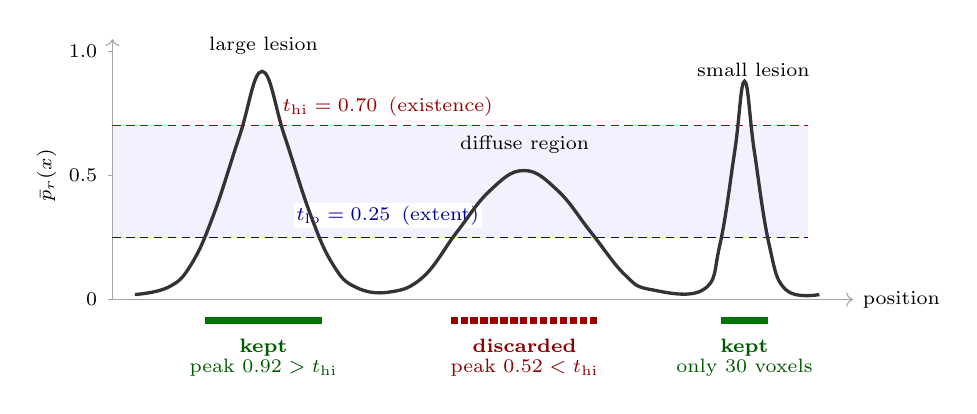
\begin{tikzpicture}[xscale=0.95, yscale=3.15]

% ---- threshold bands -------------------------------------------------------
\fill[blue!5]  (0,0.25) rectangle (9.3,0.70);

% ---- axes ------------------------------------------------------------------
\draw[->,gray!70] (0,0) -- (9.9,0) node[right,black,font=\scriptsize] {position};
\draw[->,gray!70] (0,0) -- (0,1.05);
\foreach \y/\l in {0/0, 0.5/0.5, 1.0/1.0}
  \draw[gray!70] (-0.06,\y) -- (0,\y) node[left,black,font=\scriptsize,xshift=-2pt] {\l};
\node[rotate=90,font=\scriptsize,anchor=south] at (-0.62,0.5) {$\bar{p}_r(x)$};

% ---- thresholds (labelled in the empty gap between the first two lesions) ---
\draw[densely dashed,red!70!black]  (0,0.70) -- (9.3,0.70);
\draw[densely dashed,blue!70!black] (0,0.25) -- (9.3,0.25);
\node[font=\scriptsize,red!60!black,anchor=south,fill=white,inner sep=1pt]
  at (3.68,0.725) {$t_{\mathrm{hi}}=0.70$ \,(existence)};
\node[font=\scriptsize,blue!60!black,anchor=south,fill=white,inner sep=1pt]
  at (3.68,0.285) {$t_{\mathrm{lo}}=0.25$ \,(extent)};

% ---- probability profile ---------------------------------------------------
\draw[very thick,black!80] plot[smooth,tension=0.7] coordinates {
  (0.30,0.02) (0.75,0.05) (1.05,0.14) (1.35,0.34) (1.70,0.66) (2.00,0.92)
  (2.30,0.66) (2.65,0.34) (2.95,0.14) (3.25,0.05) (3.70,0.03)
  (4.15,0.09) (4.60,0.27) (5.05,0.44) (5.50,0.52) (5.95,0.44) (6.40,0.27)
  (6.85,0.10) (7.20,0.04)
  (7.90,0.04) (8.12,0.22) (8.32,0.60) (8.45,0.88) (8.58,0.60) (8.78,0.22)
  (9.00,0.04) (9.45,0.02) };

% ---- retained / discarded extents ------------------------------------------
\draw[line width=2.6pt,green!45!black] (1.24,-0.085) -- (2.80,-0.085);
\draw[line width=2.6pt,red!60!black,densely dotted] (4.52,-0.085) -- (6.50,-0.085);
\draw[line width=2.6pt,green!45!black] (8.13,-0.085) -- (8.77,-0.085);

% ---- annotations -----------------------------------------------------------
\node[font=\scriptsize,align=center,green!35!black] at (2.02,-0.235)
  {\textbf{kept}\\[-1pt] peak $0.92>t_{\mathrm{hi}}$};
\node[font=\scriptsize,align=center,red!55!black] at (5.51,-0.235)
  {\textbf{discarded}\\[-1pt] peak $0.52<t_{\mathrm{hi}}$};
\node[font=\scriptsize,align=center,green!35!black] at (8.45,-0.235)
  {\textbf{kept}\\[-1pt] only 30 voxels};

\node[font=\scriptsize,anchor=south] at (2.02,0.95) {large lesion};
\node[font=\scriptsize,anchor=south] at (5.51,0.55) {diffuse region};
\node[font=\scriptsize,anchor=south east] at (9.45,0.86) {small lesion};

\end{tikzpicture}
\caption{Hysteresis decoding on a 1-D slice through the fused probability map; the shaded band
spans $t_{\mathrm{lo}}$ to $t_{\mathrm{hi}}$. Thresholding at $t_{\mathrm{hi}}$ alone would keep only the peaks above the band,
amputating each lesion's margin; at $t_{\mathrm{lo}}$ alone it would admit the diffuse region. Hysteresis keeps
every component of $\bar{p}_r>t_{\mathrm{lo}}$ whose peak clears $t_{\mathrm{hi}}$, at full $t_{\mathrm{lo}}$-extent (green), and drops
those that never do (red). Size is never consulted, so the 30-voxel lesion survives on one
confident voxel while the far larger diffuse region does not.}
\label{fig:hyst}
\end{figure}

The critical property is what the rule does \emph{not} use. It thresholds on peak probability and
never on component size or mean probability. This is what separates it from the component filters
that fail here (Section~\ref{sec:fp}): size and mean confidence both correlate with \emph{being a
small true lesion}, so filtering on them preferentially destroys the targets the task rewards,
whereas peak probability does not. A thirty-voxel metastasis with a single voxel at 0.9 survives
intact; a large diffuse region never reaching 0.7 anywhere is removed in full. Under this decoding rule, one confident voxel is sufficient to retain a component, while the
lower threshold determines its spatial extent.

Hysteresis is applied per region to WT, TC and ET, and excluded for RC.

\subsection{Final pipeline and reproducibility}

\begin{figure}[t]
\centering
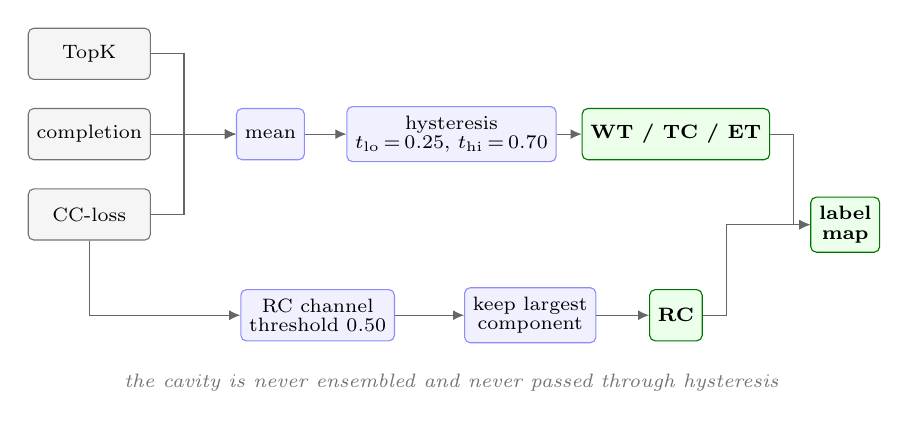
\begin{tikzpicture}[
  font=\scriptsize,
  box/.style   = {draw=black!55, rounded corners=2pt, align=center,
                  minimum height=6.5mm, inner xsep=3pt, fill=white},
  model/.style = {box, fill=black!4, minimum width=15.5mm},
  op/.style    = {box, fill=blue!6, draw=blue!45},
  fin/.style   = {box, fill=green!8, draw=green!45!black, font=\scriptsize\bfseries},
  ar/.style    = {-{Latex[length=4pt,width=3.6pt]}, draw=black!60},
]

% ---- ensemble members ------------------------------------------------------
\node[model] (m1) at (0,1.02)  {TopK};
\node[model] (m2) at (0,0)     {completion};
\node[model] (m3) at (0,-1.02) {CC-loss};

% ---- tumour path -----------------------------------------------------------
\node[op]  (mean) at (2.30,0)   {mean};
\node[op]  (hyst) at (4.60,0)   {hysteresis\\[-1pt] $t_{\mathrm{lo}}\,{=}\,0.25$, $t_{\mathrm{hi}}\,{=}\,0.70$};
\node[fin] (tum)  at (7.45,0)   {WT / TC / ET};

\draw[ar] (m1.east) -- ++(0.42,0) |- (mean.west);
\draw[ar] (m2.east) -- (mean.west);
\draw[ar] (m3.east) -- ++(0.42,0) |- (mean.west);
\draw[ar] (mean) -- (hyst);
\draw[ar] (hyst) -- (tum);

% ---- cavity path -----------------------------------------------------------
\node[op]  (rcth)  at (2.90,-2.30) {RC channel\\[-1pt] threshold $0.50$};
\node[op]  (rckp)  at (5.60,-2.30) {keep largest\\[-1pt] component};
\node[fin] (rc)    at (7.45,-2.30) {RC};

\draw[ar] (m3.south) |- (rcth.west);
\draw[ar] (rcth) -- (rckp);
\draw[ar] (rckp) -- (rc);

% ---- merge -----------------------------------------------------------------
\node[fin] (seg) at (9.60,-1.15) {label\\[-1pt] map};
\draw[ar] (tum.east) -- ++(0.30,0) |- (seg.west);
\draw[ar] (rc.east)  -- ++(0.30,0) |- (seg.west);

\node[align=center,black!55] at (4.60,-3.15)
  {\itshape the cavity is never ensembled and never passed through hysteresis};

\end{tikzpicture}
\caption{The submitted pipeline. Tumour regions are the unweighted mean of three members'
probability maps decoded by hysteresis; the cavity comes from the CC-loss member alone. The two
compose into one label map by painting WT, TC, ET, then RC, so nested regions overwrite parents.}
\label{fig:pipeline}
\end{figure}

Both thresholds were selected on the local harness of Section~\ref{sec:harness} and confirmed on
the official validation set. All code, the exact decode, the container definition and the
diagnostic scripts behind every number in this paper are released. Inference is deterministic
given the checkpoints; the submitted container bakes in all three and requires approximately
22\,s per case on the GPU used for submission testing.
% REVIEW TODO: Replace this with the exact GPU model and state whether timing includes preprocessing.

%%%%%%%%%%%%%%%%%%%%%%%%%%%%%%%%%%%%%%%%%%%%%%%%%%%%%%%%%%%%%%%%%%%%%%%%%%%%%%%
\section{Results}
\label{sec:results}

\subsection{Validation performance}

Table~\ref{tab:final} reports our best submission on the 179-case official validation set.

\begin{table}[t]
\centering
\caption{Best validation submission: three-way fusion, hysteresis $t_{\mathrm{lo}}=0.25$, $t_{\mathrm{hi}}=0.70$.
Official lesion-wise metrics, 179 cases.}
\label{tab:final}
\begin{tabular}{@{}lcccc@{}}
\toprule
 & WT & TC & ET & RC \\
\midrule
Lesion-wise Dice     & 0.725 & 0.766 & 0.746 & 0.630 \\
Lesion-wise NSD      & 0.741 & 0.815 & 0.806 & 0.521 \\
Small-instance $F_1$ & 0.376 & 0.478 & 0.476 & 0.167 \\
\bottomrule
\end{tabular}
\end{table}

Performance is markedly uneven across metric families. Overlap and surface metrics are strong,
while the three tumour $F_1$ cells sit far below at 0.376 to 0.478: indicating substantial missed and spurious detections even where matched lesions are reasonably
well delineated. Detection is therefore the dominant residual problem for the tumour regions.

\paragraph{On uncertainty and significance.} We report point estimates without confidence
intervals, which is a genuine limitation rather than an oversight: the challenge server returns
only aggregate validation scores, and per-case metrics and reference labels are withheld from
participants, so dispersion and paired significance tests cannot be computed there at all. Where we control the evaluation, we report per-case counts instead. We therefore avoid treating
small aggregate differences as evidence of statistically meaningful superiority.

\subsection{Development sequence}
\label{sec:ablation}

\begin{table}[t]
\centering
\caption{Development path. All rows are our own submissions scored on the official 179-case
validation set, and are therefore directly comparable.}
\label{tab:ablation}
\begin{tabular}{@{}llcc@{}}
\toprule
 & change & Dice WT/TC/ET & $F_1$ WT/TC/ET \\
\midrule
1 & baseline nnU-Net ResEnc-L      & 0.560/0.622/0.593 & 0.379/0.469/0.463 \\
2 & \textbf{+ ensembling}          & 0.666/0.708/0.684 & 0.368/0.439/0.436 \\
3 & + second member, step 0.25     & 0.678/0.718/0.696 & 0.370/0.477/0.484 \\
4 & + RC from the CC-loss member   & 0.679/0.719/0.696 & 0.370/0.477/0.484 \\
5 & \textbf{+ hysteresis}          & 0.711/0.753/0.729 & 0.365/0.468/0.475 \\
6 & + third member                 & 0.720/0.761/0.737 & 0.376/0.479/0.477 \\
7 & + extent $t_{\mathrm{lo}}$ 0.30 $\to$ 0.25  & \textbf{0.725/0.766/0.746} & 0.376/0.478/0.476 \\
\bottomrule
\end{tabular}
\end{table}

% REVIEW TODO: Clarify what is ensembled in row 2 and why row 3 is labelled 'second member'.
% As written, the sequence cannot be reconstructed by a reader.
This table is a sequential development trace rather than a factorial ablation, so each row-to-row
change is conditional on the preceding configuration. Two steps dominate Table~\ref{tab:ablation}. Ensembling contributes $+0.106/+0.086/+0.091$ Dice
and hysteresis a further $+0.032/+0.034/+0.033$; together they account for $+0.138/+0.120/+0.124$
of the $+0.165/+0.144/+0.153$ total, or over four fifths of it. Both are inference-time operations
on frozen probability maps. The tumour $F_1$ column tells a complementary story: neither step
improves it, and the detection gains arrive only with the high-recall third member, which is
precisely the tension Section~\ref{sec:frontier} quantifies. Over the same period the components that cost most
to develop contributed nothing that survived. A tumour-specialist and a cavity-specialist model
were each \emph{worse} than the general network at their own speciality. A distance/boundary
loss, Laplacian-of-Gaussian hint channels, MedNeXt-v2, KiU-Net, U-Mamba and larger kernels were
all abandoned after failing to beat the baseline. We also determined that ``ResEnc-XL'' and
``ResEnc-L'' instantiate an identical network for this dataset, the planners differing only in
memory target, so architecture scaling is not a decorrelation lever here.

\subsection{The Dice--$F_1$ trade-off}
\label{sec:frontier}

Interpolating the fusion weight of the high-recall CC-loss member produced a monotone trade-off
over the tested weights
(Table~\ref{tab:frontier}). $F_1$ can be bought, but only by paying Dice, and the exchange rate is
unfavourable: moving from weight $1/3$ to $1/2$ buys $+0.053/+0.051/+0.066$ $F_1$ at a cost of
$-0.050/-0.046/-0.046$ Dice across the three tumour regions. We retained $1/3$ because it gave the best overall balance
across the 12 reported region--metric cells among the tested settings; this is not intended to
reproduce the organisers' final ranking procedure.

\begin{table}[t]
\centering
\caption{Fusion weight of the CC-loss member, on the official validation set. Across the tested weights, gains in detection were accompanied by lower Dice.}
\label{tab:frontier}
\begin{tabular}{@{}lcc@{}}
\toprule
CC-loss weight & Dice WT/TC/ET & $F_1$ WT/TC/ET \\
\midrule
$1/3$ (before $t_{\mathrm{lo}}$ refinement) & \textbf{0.720/0.761/0.737} & 0.376/0.479/0.477 \\
$0.42$            & 0.695/0.738/0.714 & 0.403/0.504/0.510 \\
$1/2$             & 0.670/0.715/0.691 & \textbf{0.429/0.530/0.543} \\
\bottomrule
\end{tabular}
\end{table}

The same trade separates our two thresholds, which are \emph{not} interchangeable knobs. Lowering
the seed threshold $t_{\mathrm{hi}}$ from 0.70 to 0.65 gained $F_1$ $+0.042/+0.039/+0.043$ and lost Dice
$-0.017$ in mean tumour Dice: a large move along the trade-off, and one we rejected. Lowering the extent threshold
$t_{\mathrm{lo}}$ from 0.30 to 0.25 gained Dice $+0.005/+0.005/+0.009$ for approximately $-0.001$ mean $F_1$: a favourable change over the tested setting, and the configuration we submitted. Pushing further to
$t_{\mathrm{lo}}=0.20$ returned to trading, adding $+0.003/+0.002/+0.002$ Dice for $-0.003$ WT $F_1$, which brackets the useful range of the extent threshold at $t_{\mathrm{lo}}=0.25$.

%%%%%%%%%%%%%%%%%%%%%%%%%%%%%%%%%%%%%%%%%%%%%%%%%%%%%%%%%%%%%%%%%%%%%%%%%%%%%%%
\section{Discussion}
\label{sec:discussion}

\subsection{Confidence does not separate false positives from missed lesions}
\label{sec:fp}

On 80 training cases evaluated with the official matching code, the median peak probability of a
false-positive component was \textbf{0.96}, whereas the median maximum probability within a missed
reference lesion was \textbf{0.55}. We detected 45\% of small lesions; in 43\% of the misses, the
probability did not exceed 0.10 anywhere within the reference component. In addition, 86\% of
false-positive components were beyond the pre-specified proximity threshold from any reference
lesion.
% REVIEW TODO: Define the small-lesion criterion, the proximity threshold, the regions pooled, and
% whether these statistics use the final ensemble before or after hysteresis.

The false-positive components that survive decoding therefore have substantially higher peaks
than the reference lesions still missed by the model. They are also spatially coherent (remaining
solid after Gaussian smoothing), isolated and often corroborated across the three independently
trained networks.

We evaluated seven suppression strategies (Table~\ref{tab:suppression}) spanning post-hoc
component filtering, loss-level interventions and seed-threshold variants. None provided a useful
separation between false positives and true lesions in our experiments. This does not rule out all
confidence- or size-aware methods, but it indicates that the simple component-level criteria we
tested are poor discriminants for these models. Two failure modes were especially clear: the
per-component loss penalty produced global under-confidence, while the learned veto removed true
and false components together.

\begin{table}[t]
\centering
\caption{Seven suppression strategies evaluated. Across post-hoc, loss-level and
seed-threshold interventions, none separated false-positive components from true lesions without
a substantial detection cost in our experiments.}
\label{tab:suppression}
\small
\setlength{\tabcolsep}{4pt}
\renewcommand{\arraystretch}{1.12}
\begin{tabular}{@{}>{\raggedright\arraybackslash}p{0.335\textwidth}
                  >{\raggedright\arraybackslash}p{0.615\textwidth}@{}}
\toprule
\rowcolor{hdrrow}
\textbf{mechanism} & \textbf{outcome} \\
\midrule
\rowcolor{famrow}
\multicolumn{2}{@{}l}{\textcolor{famtext}{\emph{(a) Post-hoc component filters}: rank on size or mean confidence}}\\
\addlinespace[2pt]
small-component filters      & substantially reduced $F_1$ by removing small true lesions \\
rejection by mean confidence & increased Dice but substantially reduced recall \\
\midrule
\rowcolor{famrow}
\multicolumn{2}{@{}l}{\textcolor{famtext}{\emph{(b) Loss-level suppression}: rank on a learned per-component score}}\\
\addlinespace[2pt]
per-component FP penalty     & FP $-53\%$ but TP $-24\%$; collapsed into global under-confidence \\
the same model as a veto     & at $t=0.5$ it rejected \emph{everything} (TP $1.82\to0.51$) \\
blending the veto with the base & FPs and TPs removed in lockstep at every mixing ratio \\
\midrule
\rowcolor{famrow}
\multicolumn{2}{@{}l}{\textcolor{famtext}{\emph{(c) Seed-threshold variants}: rank on a transformed confidence}}\\
\addlinespace[2pt]
size-adaptive seed threshold & reproduces the plain global threshold exactly \\
scale-space (smoothed) seed  & at every matched FP rate the plain threshold detects more \\
\bottomrule
\end{tabular}
\end{table}

\subsection{False positives are consistent with anatomical mimics}

Two explanations remained. Either these are anatomical \emph{mimics} (enhancing vessels, choroid
plexus, dural structures) that a radiologist excludes using context the network lacks, or they
are \emph{real metastases the annotators missed}, in which case part of the ceiling is not ours
to move.

Non-expert visual review of the 48 most confident false positives was consistent with the mimic hypothesis. They are
overwhelmingly small bright enhancing foci in three anatomically suspicious locations: at the
cortical margin or dura, on or beside bright linear tubular structures consistent with vessels,
and at the midline in falx and superior sagittal sinus territory. Few appeared as isolated round parenchymal foci away from conspicuous anatomical structures,
although this distinction cannot be established reliably without expert review.

That review was carried out by a non-radiologist on single axial slices, so we treated it as a
hypothesis to test rather than a clinical assessment. Anatomical position is a genuinely
different separation axis from confidence, so we measured it. Distance from the brain surface to the false-positive
centroid has a median of 8.8\,mm against 11.2\,mm for reference lesion centroids, with almost
fully overlapping interquartile ranges and an area under the ROC curve of \textbf{0.575}. False
positives are only marginally more peripheral, and grey--white junction metastases, a common
true presentation, sit at the same depth, so surface proximity alone is unlikely to remove many suspected mimics without also removing real lesions. The measurement is worth reporting precisely because the
hypothesis is attractive: anatomical context is the obvious thing a radiologist uses and a network
lacks, and this result suggests that any useful anatomical discriminator would need to be substantially more
specific than raw surface proximity.

\subsection{What target-level intervention buys, and what it costs}

Since decoding could not separate these errors, we attacked the 43\% of misses to which the
network is wholly blind from the training side.

\paragraph{Sampling frequency is not the bottleneck.} nnU-Net's sampler draws a random key from
\texttt{class\_locations} and then a random voxel within it, so a thirty-voxel metastasis sharing
a key with every large-lesion and oedema voxel is patch-centred approximately 0.3\% of the time.
We added a dedicated key containing only small-component voxels, with every lesion weighted
equally regardless of size. Verified over 4000 draws, the probability of centring a patch on a
small lesion rose from 1.28\% to 25.75\%, a twenty-fold increase. Small-lesion detection did not improve materially. This suggests that patch-sampling frequency was
not the primary cause of the observed misses in this experiment.

\paragraph{Enlarging the target does find more lesions, at a price the metric sets.} We instead dilated isolated
small targets, so a thirty-voxel lesion presents roughly four times the volume and a larger
object for the receptive field, with a matched selective erosion at inference. Submitted alone
this lifted tumour $F_1$ by $+0.012/+0.014/+0.013$, evidence that a meaningful share of the extra
detections are real. Grafting only the additional, non-overlapping detections onto our best
submission raised $F_1$ by as much as $+0.034/+0.027/+0.031$ but lowered lesion-wise Dice by
$-0.010/-0.012/-0.012$. The overall balance across the reported metrics was negative for our selected operating point. The reason is specific to lesion-wise scoring and
worth stating plainly: \emph{many newly detected small lesions entered the per-lesion Dice average at a below-average value}, because small lesions are segmented less accurately than large ones.
Under volumetric Dice these small components would receive much less weight; under lesion-wise
Dice they contribute equally. A more
aggressive variant added 156 further components averaging six voxels each and bought only
$+0.003/+0.004/+0.005$ $F_1$, indicating that most of these very small additional components were false positives.

\subsection{Lessons for lesion-wise post-processing validation}
\label{sec:harness}

We built a local harness around the official evaluation code using 80 reference tumour cases and
100 cavity cases. Because every model had been trained on these cases, this harness was not an
unbiased estimate of generalisation. We used it only as a ranking heuristic and first required it
to reproduce the relative ordering of our own previously scored submissions. It then allowed us
to compare 28 candidate decodes without consuming additional submissions.

The rankings transferred reasonably for the threshold and fusion settings we tested, but failed
for a rule that explicitly retained additional cavity components. On memorised cases, spurious
components were uncommon, so the rule appeared to add true positives with little false-positive
cost. On unseen validation data, the same rule also admitted spurious components. A cavity
keep-rule estimated locally at $+0.028$ lesion-wise Dice instead produced $-0.016$ on official
validation, reversing the sign of the predicted effect.

This observation supports a narrower practical recommendation than a universal protocol. Results
from training-set post-processing should be treated as provisional, especially when a rule changes
component retention. A genuine held-out fold is preferable; when none exists, at least one official
submission should be reserved to validate such changes. Threshold and fusion rankings happened to
transfer better in our experiments, but training-set agreement does not guarantee held-out
improvement for those settings either.

%%%%%%%%%%%%%%%%%%%%%%%%%%%%%%%%%%%%%%%%%%%%%%%%%%%%%%%%%%%%%%%%%%%%%%%%%%%%%%%
\subsection{Conclusion}
\label{sec:conclusion}

Our BraTS 2026 Task 1 submission reaches WT/TC/ET lesion-wise Dice of
0.725/0.766/0.746 using probability averaging and hysteresis decoding without changing the
constituent network architectures. The largest remaining weakness is tumour detection. In our
models, simple confidence- and size-based suppression did not separate false-positive components
from true lesions, non-expert review suggested that many errors may be anatomical mimics, and
attempts to recover additional small lesions traded improved $F_1$ against lower lesion-wise Dice.
The main practical lesson is therefore methodological: inference-time decoding can materially
change challenge performance, while post-processing selected on cases used for training must not
be treated as evidence of held-out improvement. All code is released at
\url{https://github.com/aymuos15/brats2026-mets}.

\section*{Acknowledgements}
Data used in this publication were obtained as part of the Challenge project through Synapse ID
syn74274097.

\begin{thebibliography}{99}

\bibitem{baid2021}
Baid, U., et al.: The RSNA-ASNR-MICCAI BraTS 2021 benchmark on brain tumor segmentation and
radiogenomic classification. arXiv:2107.02314 (2021)

\bibitem{bratsmet2023}
Moawad, A.W., et al.: The Brain Tumor Segmentation (BraTS-METS) challenge 2023: brain metastasis
segmentation on pre-treatment MRI. arXiv:2306.00838 (2023)

\bibitem{bratsmet2025}
Maleki, N., et al.: Analysis of the MICCAI Brain Tumor Segmentation--Metastases (BraTS-METS) 2025
Lighthouse Challenge: brain metastasis segmentation on pre- and post-treatment MRI.
arXiv:2504.12527 (2025)

\bibitem{brats2026}
Bakas, S., et al.: BraTS 2026 Cluster of Challenges. Zenodo (2026).
\url{https://doi.org/10.5281/zenodo.19714728}

\bibitem{medperf2023}
Karargyris, A., Umeton, R., Sheller, M.J., et al.: Federated benchmarking of medical artificial
intelligence with MedPerf. Nature Machine Intelligence \textbf{5}, 799--810 (2023)

\bibitem{isensee2021nnunet}
Isensee, F., Jaeger, P.F., Kohl, S.A.A., Petersen, J., Maier-Hein, K.H.: nnU-Net: a
self-configuring method for deep learning-based biomedical image segmentation. Nature Methods
\textbf{18}(2), 203--211 (2021)

\bibitem{isensee2024resenc}
Isensee, F., et al.: nnU-Net revisited: a call for rigorous validation in 3D medical image
segmentation. In: MICCAI 2024. Springer (2024)

\bibitem{kofler2022blob}
Kofler, F., et al.: blob loss: instance imbalance aware loss functions for semantic segmentation.
In: IPMI 2023. Springer (2023)

\bibitem{canny1986}
Canny, J.: A computational approach to edge detection. IEEE Transactions on Pattern Analysis and
Machine Intelligence \textbf{8}(6), 679--698 (1986)

\bibitem{kundu2026instance}
Kundu, S.S., Kofler, F., Ivory, M., M\"oller, H., Shapey, J., Vercauteren, T.: Instance awareness
of multi-class semantic segmentation loss functions. arXiv:2604.24276 (2026)

\bibitem{grosskopf2026matching}
Gro\ss{}kopf, E., Kundu, S.S., M\"oller, H., M\"unster, N., Astaraki, M., Buzduga, P.T., Ritter, K.,
Wiestler, B., Kirschke, J., Shapey, J., Vercauteren, T., Kofler, F.: Redefining instance matching:
a unified framework for part-aware matching in panoptic segmentation evaluation.
arXiv:2605.31094 (2026)

% REVIEW TODO: Verify the exact organiser-mandated citation list immediately before submission.

\end{thebibliography}

\end{document}
